\section{Feature Engineering}
\label{sec:feature_engineering}
Good features are critical for machine learning based methods to work.
Intuitively, good features have better and deeper understanding of properties
of the optimization tasks. Basic pre-processing, like standardization, mean
removal, variance scaling, are not sufficient for our task of predicting real
world network bandwidth.

Through experiment, we performed the following two feature engineering
procedures to boost the regression accuracy: sequence smoothing, and Fourier
transformation.

\subsection{Sequence Smoothing}
\label{sub:sequence_smoothing}
Noise is recognized as a potential issue for bandwidth estimation in practice,
as in Figure~\ref{fig:smoothing}, noise together with interrupt coalescing
can make the receiving signal very hard to convey effective information.
Different smoothing strategies have been proposed to suppress the noise in
probing results. We adopted \cite{Yin2014} as the smoothing method. We only
used the first pass of the smoothed data for noise removal purposes.

As can be seen in Figure~\ref{fig:smoothing:recv}, striking peaks have been
removed from the smoothed receiving signal. Such regular data are a lot easier
to train and optimize.

\begin{figure}[htpb]
   \centering
   \subfloat[Send gaps]{
      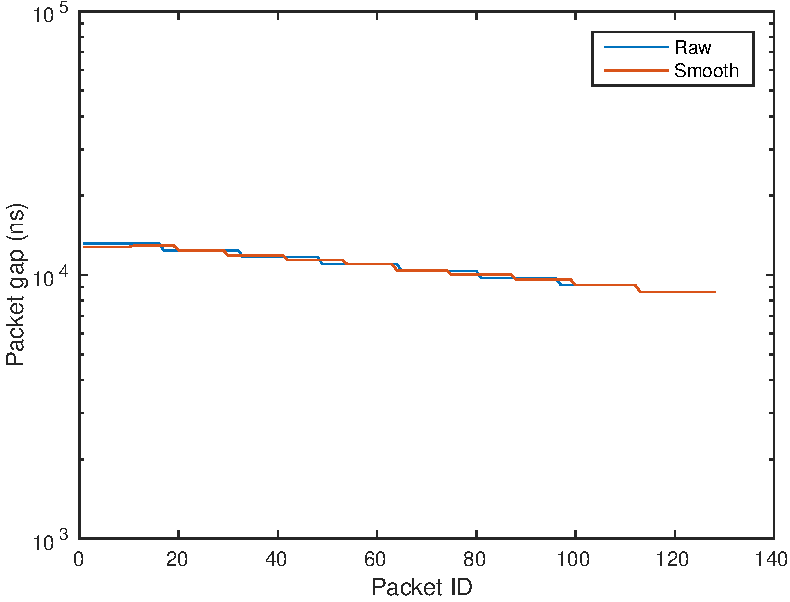
\includegraphics[width=0.45\linewidth]{figures/smooth_send.pdf}
   }
   \quad
   \subfloat[Received gaps]{
      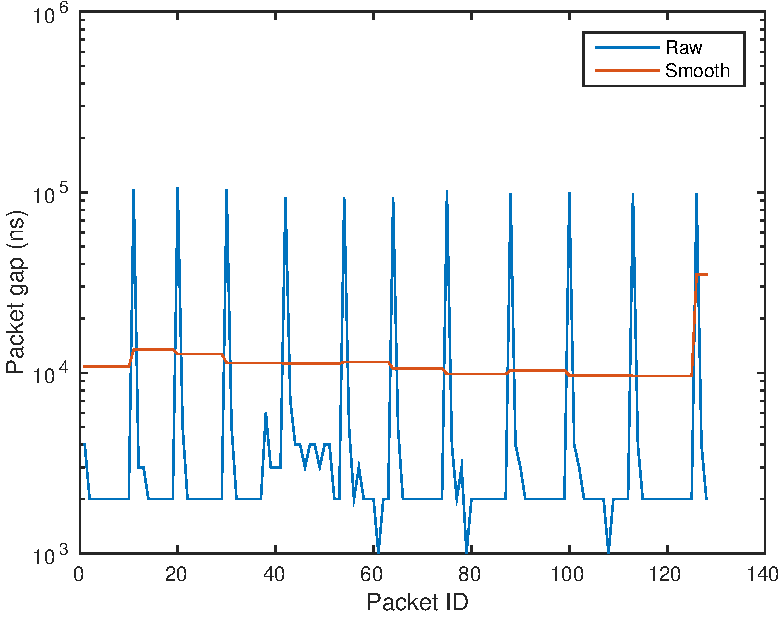
\includegraphics[width=0.45\linewidth]{figures/smooth_recv.pdf}
      \label{fig:smoothing:recv}
   }
   \caption{Smoothing raw packet gaps.}
   \label{fig:smoothing}
\end{figure}

\subsection{Fourier Transformation}
\label{sub:fourier_transformation}

Noise in measurements, interrupt coalesces, cross traffic over the network, can
make the received packet gaps to behave abnormally. In our experiments, we
found that the location of the peaking locations can vary because of different
reasons. If send and received gaps are concatenated as features, such
misalignment can cause confusion over the actual physical meaning of different
dimensions.

We adopted Fourier transformation to convert the feature vector to the
frequency domain to address the shifting issue. By converting the raw signal to
frequency space, such temporal shift will be neglected, thus feature vectors
can better capture the underlying models.

\begin{figure}[htpb]
   \centering
   \subfloat[Send gaps]{
      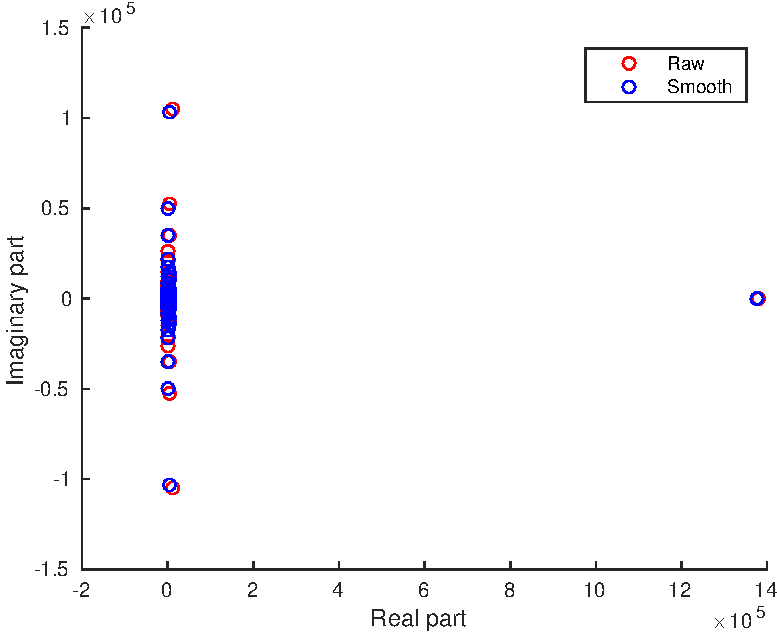
\includegraphics[width=0.45\linewidth]{figures/fft_send.pdf}
      \label{fig:fft:send}
   }
   \quad
   \subfloat[Received gaps]{
      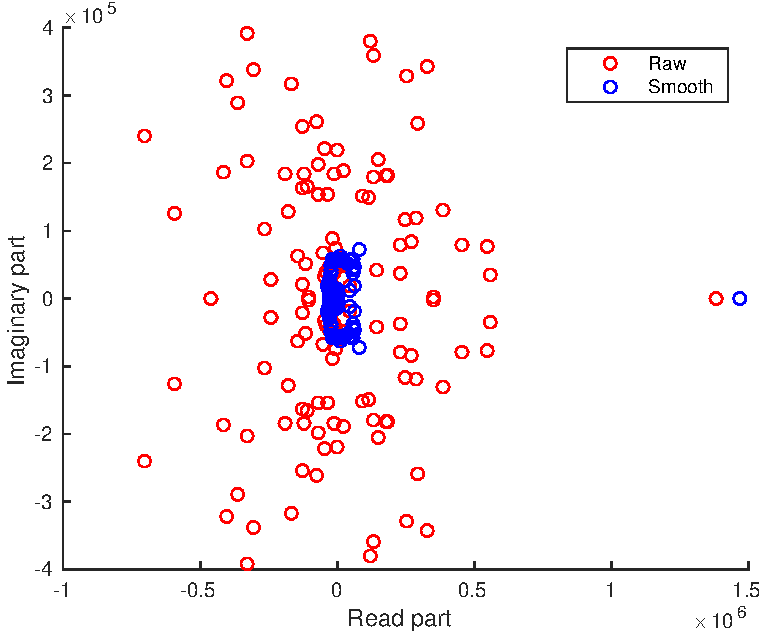
\includegraphics[width=0.45\linewidth]{figures/fft_recv.pdf}
      \label{fig:fft:recv}
   }
   \caption{Fourier transformation on raw packet gaps.}
   \label{fig:fft}
\end{figure}

We applied FFT on the raw and smooth signal in Figure~\ref{fig:smoothing} and
plotted the real and imaginary parts of the FFT coefficients in
Figure~\ref{fig:fft}. From Figure~\ref{fig:fft:recv} we can see that by
applying FFT, we convert the striking raw pattern of the received gaps to a set
of more discrete data points. Then by utilizing different learning algorithms,
we can discover the underlying relationship between such frequency coefficients
and the actual available network bandwidth. One thing worth noticing is that
smoothed receiving gaps are more centralized, which makes learning and
optimization easier. This agrees with our conclusion in
Section~\ref{ssub:accuracy} that smoothing helps boosting accuracy.

\section{Experiment}
\label{sec:experiment}
In this section, we describe our  experimental setting in
Section~\ref{sub:parameter_setting}, results and benchmarks in
Section~\ref{sub:benchmark}.
\subsection{Experimental Setting}
\label{sub:parameter_setting}
In order to test the generalization and robustness of the estimators, we
collect probing streams with different settings.
For each dataset, we specify a range of probing speed, and the number of packet
sending rate used for probing, together with the number of packets sent on a
specific rate. With a fixed setting, we collect dataset using the experimental
setting in \cite{Yin2014}. Incomplete and invalid streams are discarded.
Detailed statistics of datasets can be found in Table~\ref{tab:dataset}.

\begin{table}[htpb]
   \centering
   \caption{Dataset}
   \label{tab:dataset}
   \begin{tabular}{|c|c|c|c|c|l|l|l|l|}
      \hline
      Name & Range & \# Rate & \# Packets & Length & Total & Valid          & Training & Test\\ \hline
      Exp4 & 50\%  & 8       & 16         & 128    & 11003 & 7475(67.94\%)  & 5233     & 2242 \\
      Exp5 & 50\%  & 2       & 16         & 128    & 11003 & 7188(65.33\%)  & 5032     & 2156 \\
      Exp6 & 50\%  & 3       & 16         & 129    & 10691 & 883(8.26\%)    & 618      & 265 \\
      Exp7 & 50\%  & 6       & 16         & 126    & 11016 & 7203(65.39\%)  & 5042     & 2161 \\
      Exp8 & 50\%  & 4       & 16         & 128    & 33310 & 18185(54.59\%) & 12730    & 5455  \\ \hline
   \end{tabular}
\end{table}

In order to achieve better performance, we ran a 5 fold cross validation on the
training dataset to tune parameters of different estimators. Here are the
parameter settings we use for prediction:
\begin{itemize}
   \item AdaBoost: we used 200 decision tree regressor as base estimators. With
      learning rate of 1.0, and linear loss function, we achieved an error rate
      of 2.18\%.
   \item Elastic net: we used a smaller learning rate $\alpha=0.5$, together
      with a $L_1$ ratio $\rho=0.5$. Optimization by coordinate descent can
      converge within 50000 iterations with a threshold of $0.3$.
   \item Gradient boost: we used least squares regression as the loss function,
      with learning rate of $0.1$, 200 boosting stages. For each individual
      regression estimator, we constrain the maximum depth to be 3, minimum
      number of samples of splitting internal node to be 2, minimum number of
      samples required to be a leaf node to be 2.
   \item Lasso: we adopted a higher learning rate of $\alpha=1$. Optimization
      by coordinate descent can coverage within 10000 iterations with a
      threshold of $0.5$. With such a relatively high threshold, we can still
      achieve an average error rate of $2.03\%$.
   \item Nearest neighbor regression: we used a fix number of 10 nearest
      neighbors for the regression. Neighboring data points are weighted by
      the inverse of the distance to the query data point. In order to speed up
      searching, we adopted KD-tree as the underlying structure. Leaf node size
      is set to 30. Euclidean distance is used as distance metric.
   \item Random forest regressor: we used 10 trees to assemble the random
      forest. Mean squared error is used as the split quality measure. Minimum
      number of samples required to split an internal node is set to 2, minimum
      number of samples in newly created leaves is set to 1.
\end{itemize}

\subsection{Benchmark}
\label{sub:benchmark}

We randomly partitioned the dataset into training set (70\%) and test
set(30\%), as shown in Table~\ref{tab:dataset}. We train and cross validate
estimators on the training set, all following benchmark is performed on the
isolated test dataset.

\subsubsection{Computation Performance}
\label{ssub:computation_performance}

Our primary goal of this project is to investigate the possibility of applying
machine learning techniques to predicting available bandwidth in real world
networking experimental settings. Computation efficiency is not our primary
concentration. If learning based estimators were to be deployed in real world
networking environments, efficiency is an important factor especially for
real-time applications.

Compared with training, prediction takes considerably less amount of time and
resources. We list only average feature transformation and training time in
Table~\ref{tab:timing}.

\begin{table}[htpb]
   \centering
   \caption{Average processing time over 28655 streams.}
   \label{tab:timing}
   \begin{tabular}{|c|r|r|r|r|r|r|}
      \hline
      \multirow{2}{*}{Algorithms} & \multicolumn{2}{c|}{Feature extraction} &
      \multicolumn{4}{c|}{Training} \\ \cline{2-7}
                       & Raw   & Smooth & Raw            & Raw FFT        & Smooth         & Smooth FFT \\ \hline
      AdaBoost         & 15.71 & 14.94  & 2026.13        & 35766.15       & 13109.74       & 32991.03\\
      Elastic net      & 16.60 & 16.06  & 151.96         & 577.30         & 121.73         & 537.47\\
      Gradient boost   & 12.55 & 12.52  & 8090.82        & 45908.08       & 9695.63        & 46406.90\\
      Lasso            & 16.23 & 16.14  & 145.09         & 507.52         & 139.83         & 567.07\\
      NNR              & 15.78 & 15.59  & \textbf{18.75} & \textbf{33.29} & \textbf{18.34} & \textbf{35.41}\\
      Random forest    & 15.80 & 15.61  & 3139.64        & 9236.24        & 3207.93        & 9380.83\\
      \hline
   \end{tabular}
\end{table}

We evaluated the average accuracy over all test datasets, with 12279 probing
sequences in total. We include standard derivation of the average
accuracy in parentheses. \cite{Yin2014} has an average accuracy of 6.97\%
with standard derivation of $\sigma=0.0451$.

\subsubsection{Accuracy}
\label{ssub:accuracy}
\begin{table}[htpb]
   \centering
   %6.97
   \caption{Average accuracy of different estimators over different features.}
   \label{tab:accuracy}
   \begin{tabular}{|c|c|c|c|c|}
      \hline
      Algorithms     & Raw                     & Raw FFT                 & Smooth                  & Smooth FFT \\ \hline
      AdaBoost       & 2.82\%(0.0194)          & 2.38\%(0.0160)          & 2.29\%(0.0151)          & 2.18\%(0.0148)\\
      Elastic net    & 2.30\%(0.0159)          & 2.19\%(0.0162)          & 2.16\%(0.0145)          & 1.96\%(0.0140)\\
      Gradient boost & 2.41\%(0.0177)          & \textbf{1.96\%}(0.0144) & \textbf{1.89\%}(0.0135) & \textbf{1.82\%}(0.0134)\\
      Lasso          & 2.70\%(0.0190)          & 2.37\%(0.0172)          & 2.25\%(0.0151)          & 2.03\%(0.0146)\\
      NNR            & \textbf{2.29\%}(0.0169) & 2.29\%(0.0169)          & 2.17\%(0.0158)          & 2.17\%(0.0158)\\
      Random forest  & 2.35\%(0.0178)          & 2.01\%(0.0153)          & 2.05\%(0.0148)          & 1.89\%(0.0144)\\
      \hline
   \end{tabular}
\end{table}

We also show the prediction accuracy of each estimator over different datasets
in Figure~\ref{fig:error}. \cite{Yin2014} produces satisfying results
over different network. But as can be seen from
Figure~\ref{fig:error:adaboost}, accuracy of \cite{Yin2014} can vary across
different datasets. Comparatively, our estimators demonstrated stronger
robustness over different network settings.

For machine learning based approaches to work well, the amount and quality of
available training data are important. For example, we can see an increase in
error rate on the 3-rate datasets in Figure~\ref{fig:error:elasticnet} and
Figure~\ref{fig:error:gradientboost}. In Table~\ref{tab:dataset} this dataset
has only 8\% valid streams, leading to a smaller training set. For methods with
a larger parameter space, such method are more likely to underfit.

We tried two different feature engineering methods over the raw stream data, as
stated in Section~\ref{sub:feature_engineering}. From Figure~\ref{fig:error} we
can see that both feature engineering approaches are effective. By applying FFT
over raw sequences, we actually transformed the raw features into a temporal
invariant representation. Intuitively, this is helpful because the shifting of
peaks of raw signals(see Figure~\ref{fig:smoothing:recv} for an example) can
lead to misalignment along different dimensions of the feature vectors we
assembled. By converting the raw signal to frequency space, such temporal shift
will be neglected, thus feature vectors can better capture the underlying
models.

On the other hand, smoothing helps to boost performance by removing noise data
points in the feature vectors. By transforming the raw sequence into smooth
data, we can capture features that are more important for regression. The
smoothing procedure we applied can actually be regarded as a domain-knowledge
powered feature selection procedure.

\begin{figure}[htpb]
   \centering
   \subfloat[AdaBoost]{
      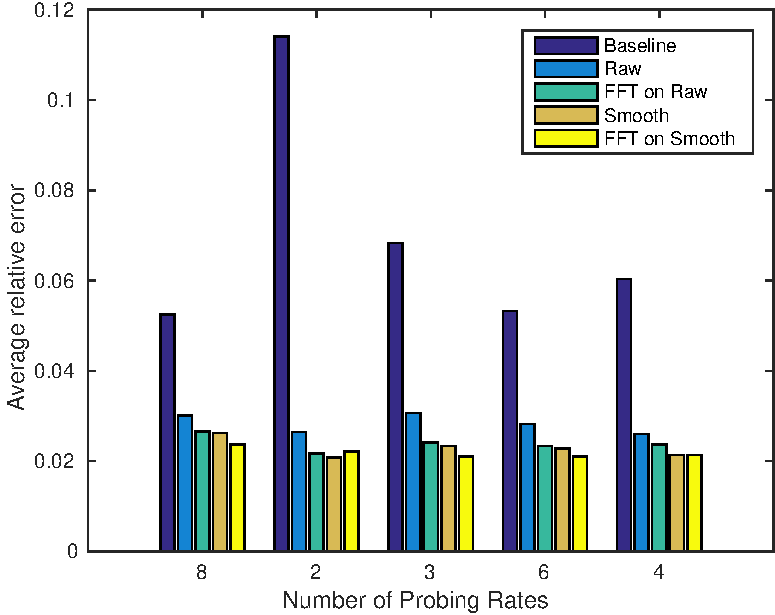
\includegraphics[width=0.3\linewidth]{figures/error_adaboost.pdf}
      \label{fig:error:adaboost}
   }
   \quad
   \subfloat[Elastic net]{
      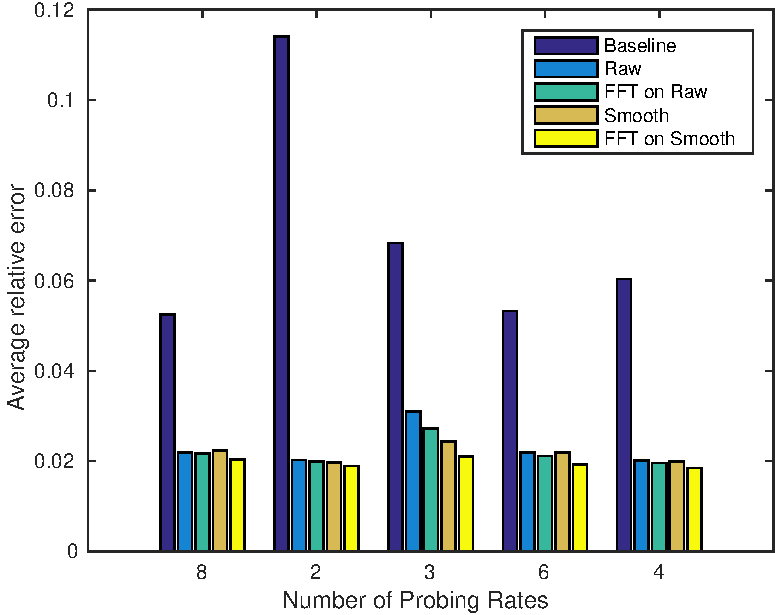
\includegraphics[width=0.3\linewidth]{figures/error_elastic_net.pdf}
      \label{fig:error:elasticnet}
   }
   \quad
   \subfloat[Gradient boost]{
      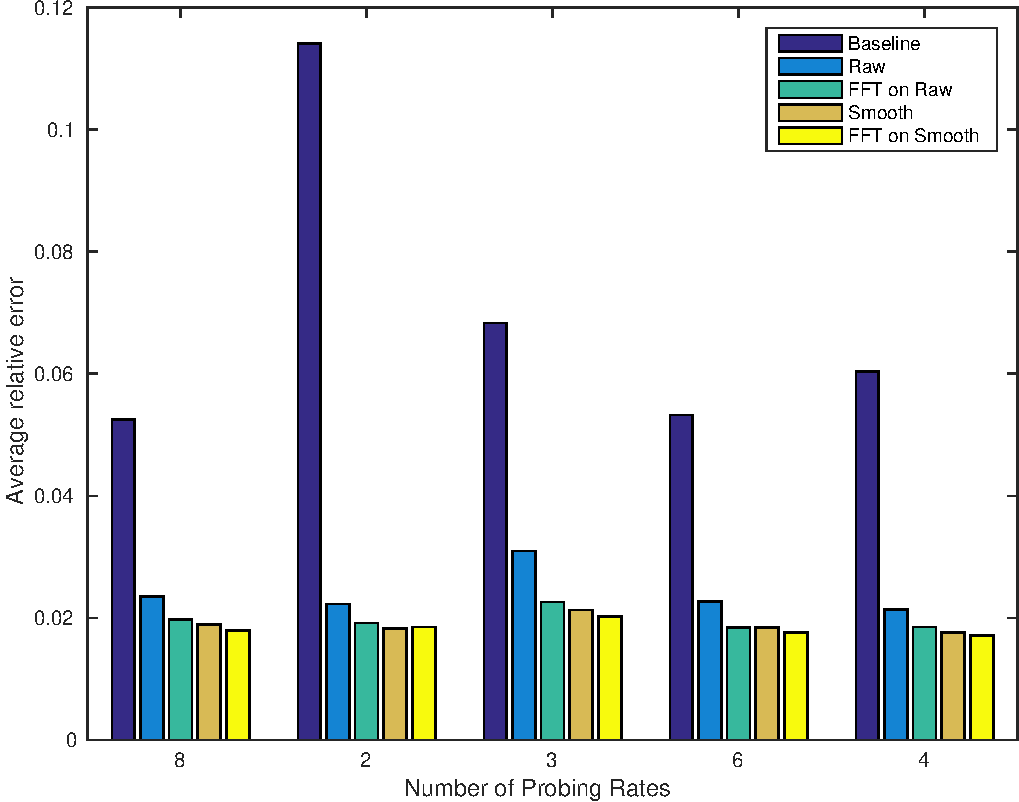
\includegraphics[width=0.3\linewidth]{figures/error_gradient_boost.pdf}
      \label{fig:error:gradientboost}
   }
   \\
   \subfloat[Lasso]{
      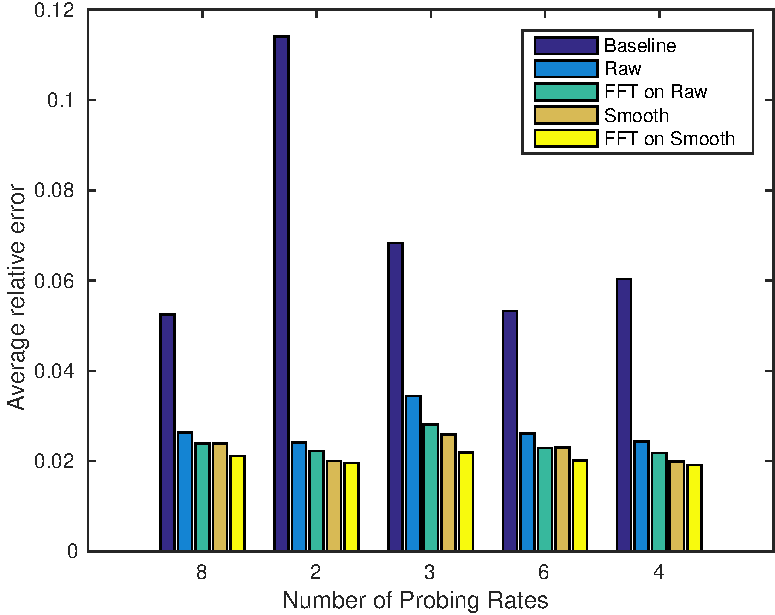
\includegraphics[width=0.3\linewidth]{figures/error_lasso.pdf}
      \label{fig:error:lasso}
   }
   \quad
   \subfloat[NNR]{
      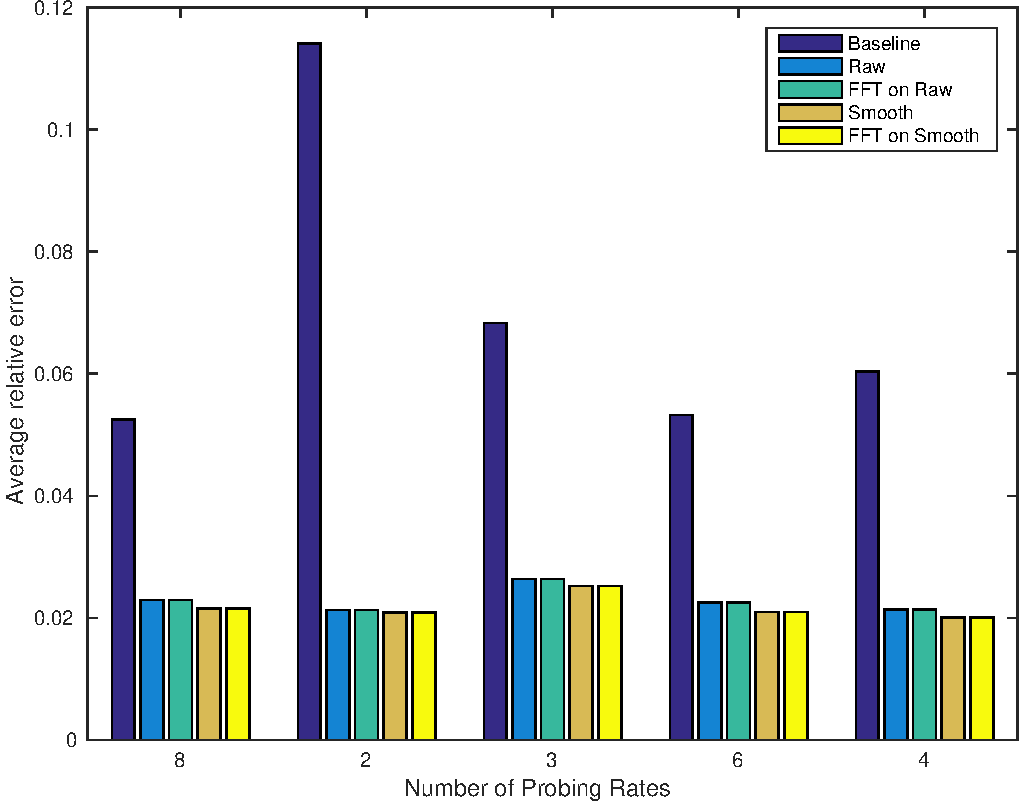
\includegraphics[width=0.3\linewidth]{figures/error_nnr.pdf}
      \label{fig:error:nnr}
   }
   \quad
   \subfloat[Random forest]{
      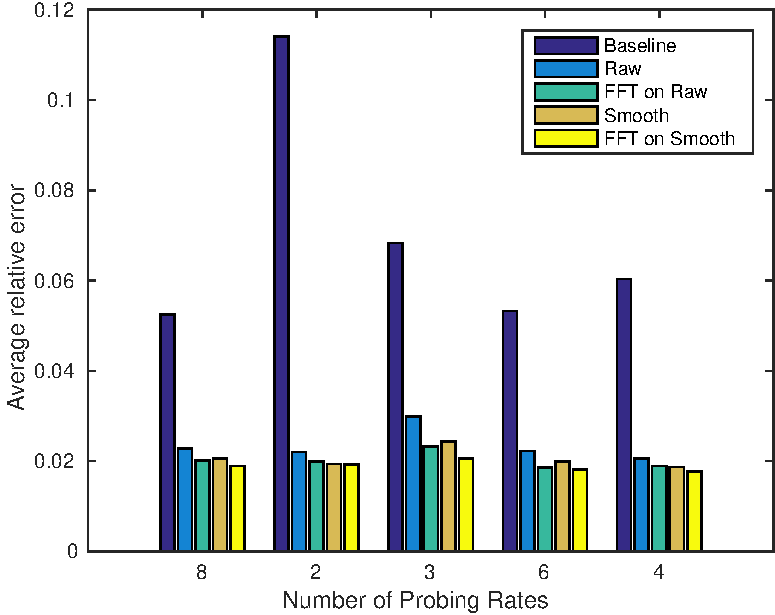
\includegraphics[width=0.3\linewidth]{figures/error_random_forest.pdf}
      \label{fig:error:randomforest}
   }
   \caption{Relative error of different estimators.}
   \label{fig:error}
\end{figure}

\begin{figure}[htpb]
   \centering
   \subfloat[AdaBoost]{
      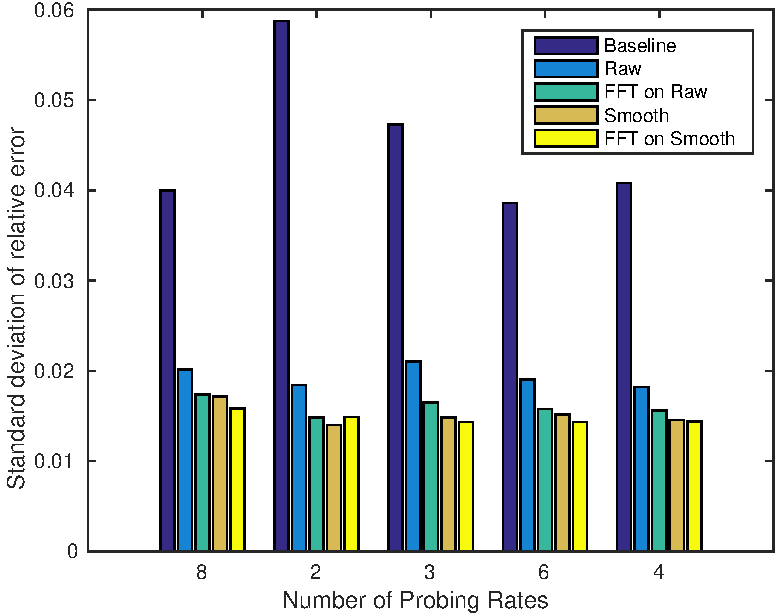
\includegraphics[width=0.3\linewidth]{figures/std_adaboost.pdf}
      \label{fig:std:adaboost}
   }
   \quad
   \subfloat[Elastic net]{
      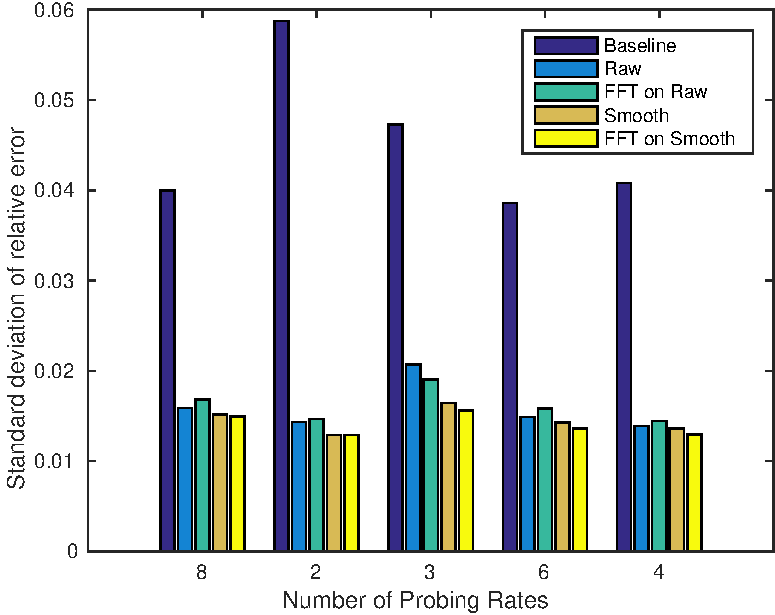
\includegraphics[width=0.3\linewidth]{figures/std_elastic_net.pdf}
      \label{fig:std:elasticnet}
   }
   \quad
   \subfloat[Gradient boost]{
      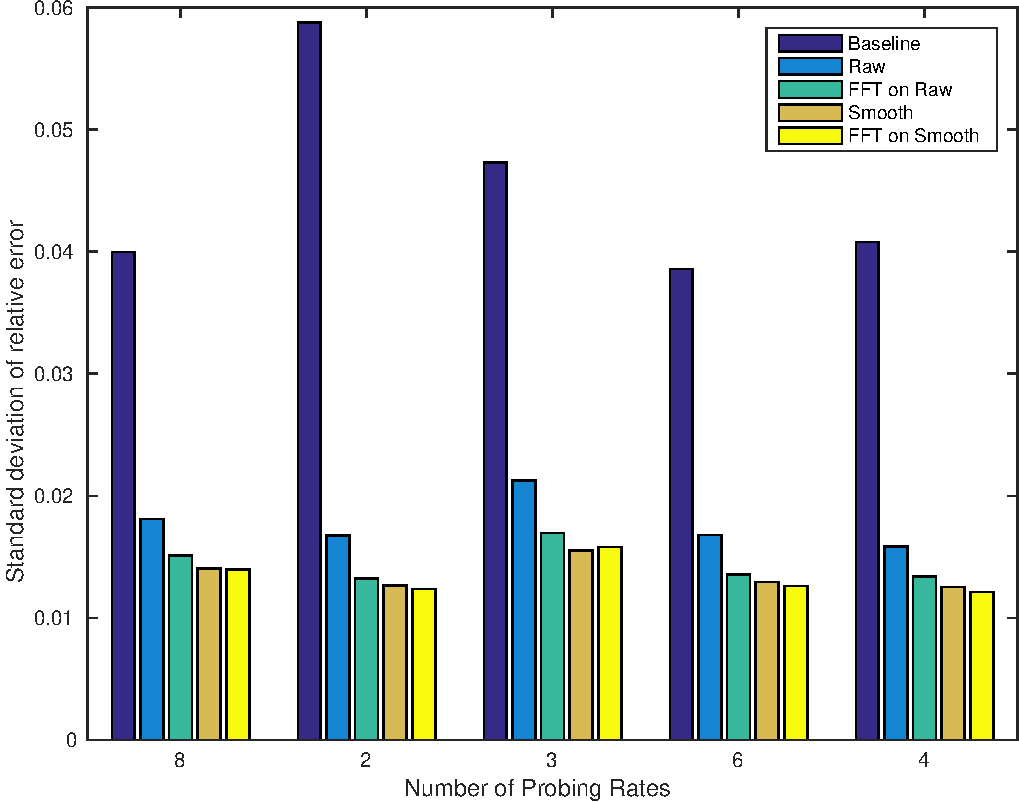
\includegraphics[width=0.3\linewidth]{figures/std_gradient_boost.pdf}
      \label{fig:std:gradientboost}
   }
   \\
   \subfloat[Lasso]{
      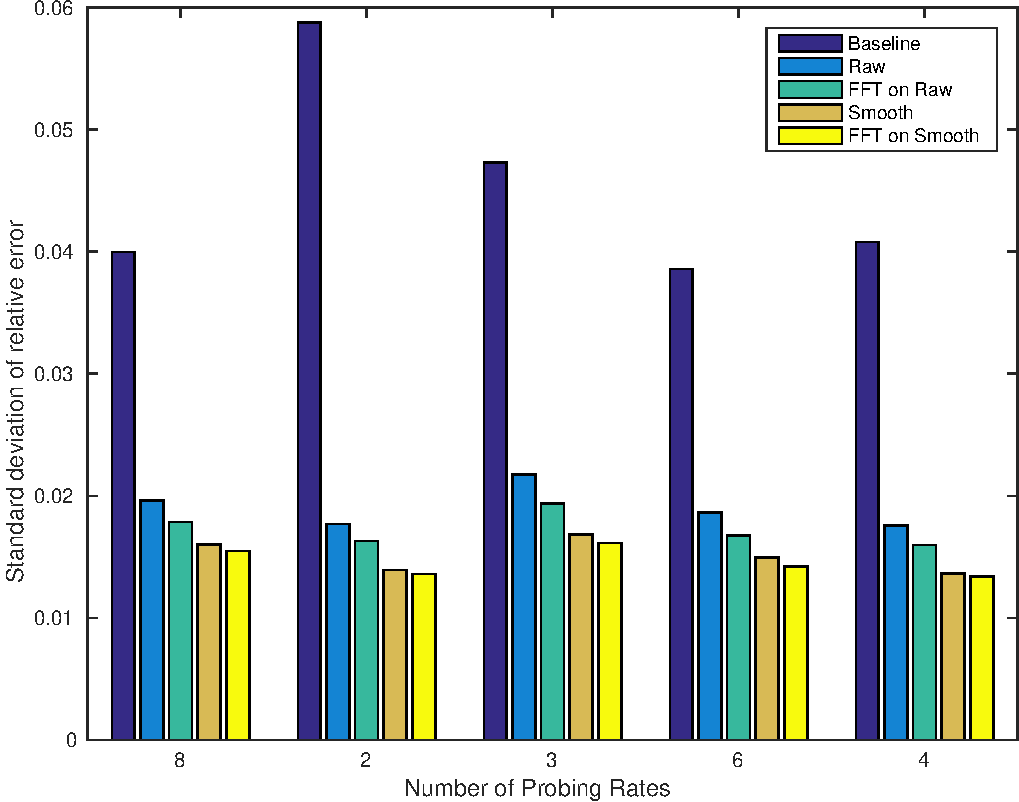
\includegraphics[width=0.3\linewidth]{figures/std_lasso.pdf}
      \label{fig:std:lasso}
   }
   \quad
   \subfloat[NNR]{
      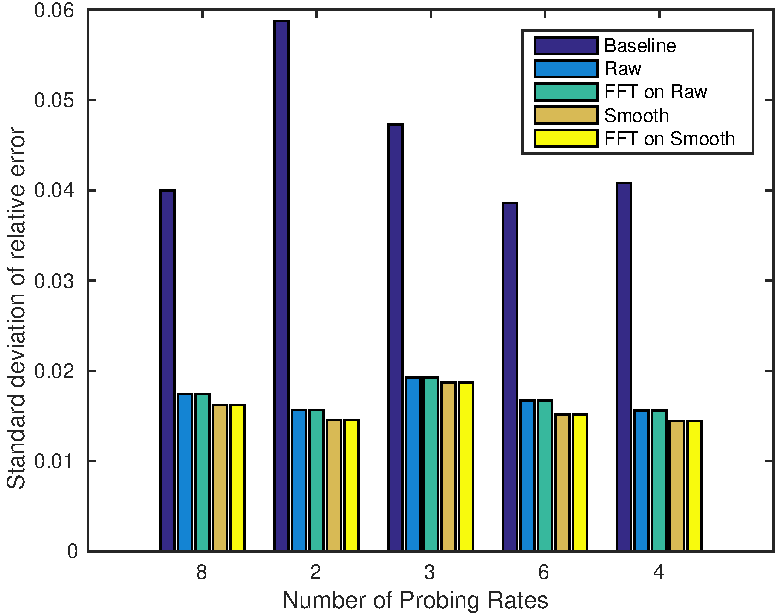
\includegraphics[width=0.3\linewidth]{figures/std_nnr.pdf}
      \label{fig:std:nnr}
   }
   \quad
   \subfloat[Random forest]{
      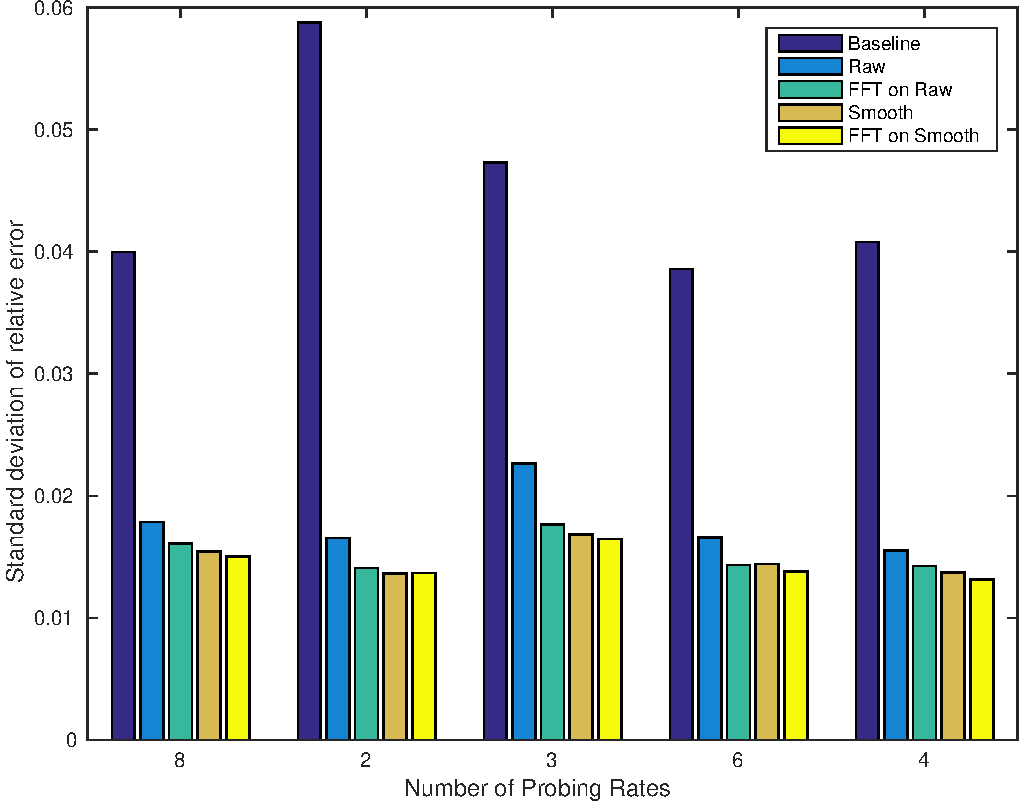
\includegraphics[width=0.3\linewidth]{figures/std_random_forest.pdf}
      \label{fig:std:randomforest}
   }
   \caption{Standard derivation on average error of different estimators.}
   \label{fig:std}
\end{figure}

To better illustrate the prediction accuracy, we overlay the histogram of
baseline prediction with our estimators on one dataset in
Figure~\ref{fig:hist}. The example dataset has 8 rates, each rate containing 16
packets. Our estimation has relatively low errors, and the prediction errors
has a much tighter distributions.

\begin{figure}[htpb]
   \centering
   \subfloat[AdaBoost]{
      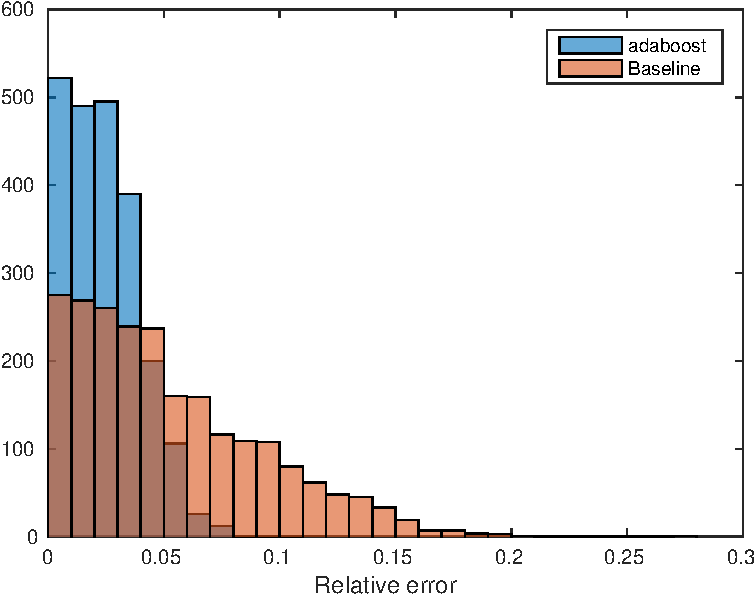
\includegraphics[width=0.3\linewidth]{figures/histogram_adaboost.pdf}
   }
   \quad
   \subfloat[Elastic net]{
      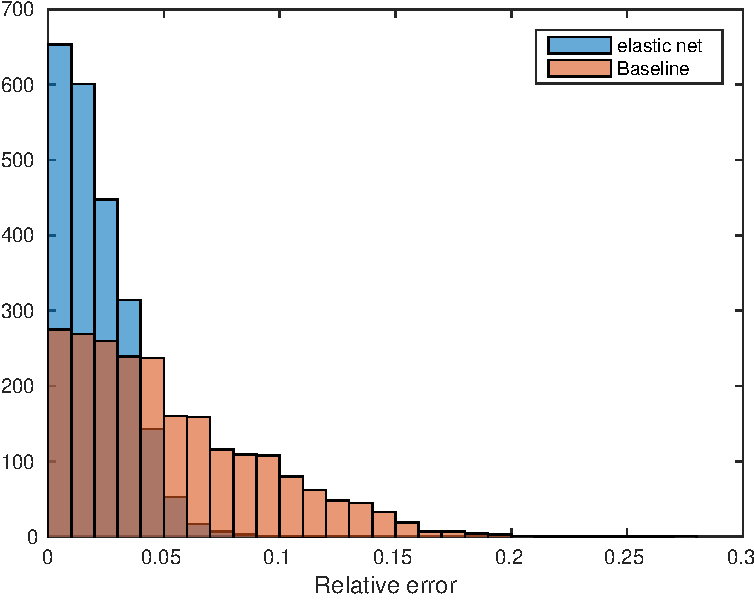
\includegraphics[width=0.3\linewidth]{figures/histogram_elastic_net.pdf}
   }
   \quad
   \subfloat[Gradient boost]{
      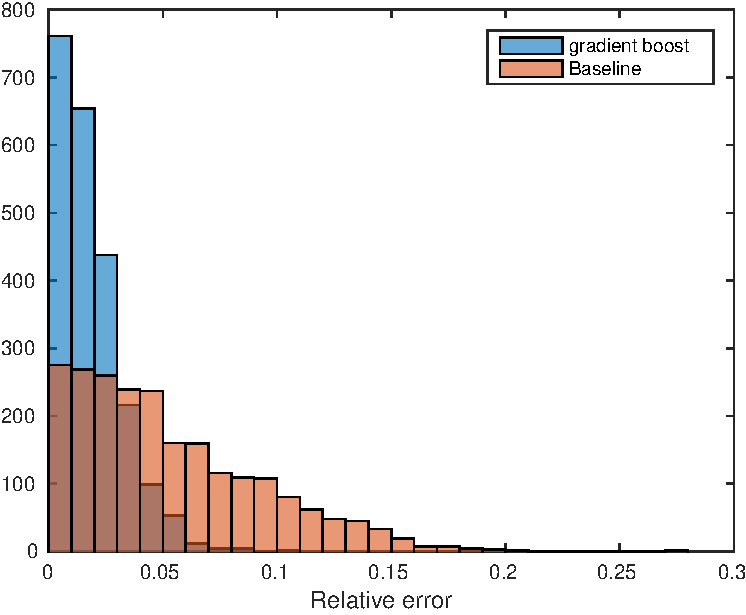
\includegraphics[width=0.3\linewidth]{figures/histogram_gradient_boost.pdf}
   }
   \\
   \subfloat[Lasso]{
      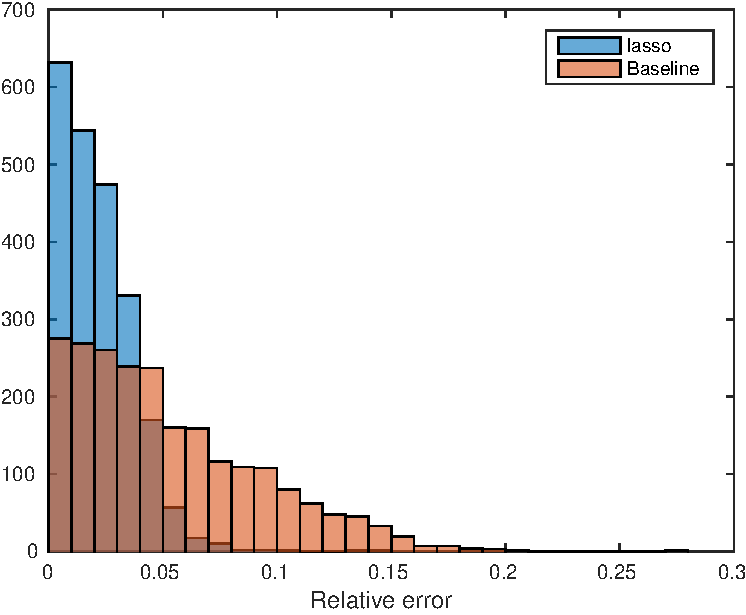
\includegraphics[width=0.3\linewidth]{figures/histogram_lasso.pdf}
   }
   \quad
   \subfloat[NNR]{
      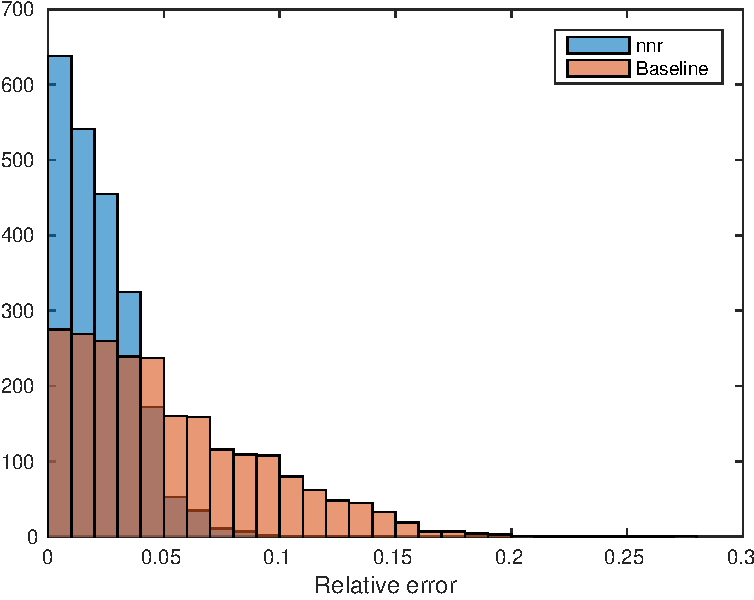
\includegraphics[width=0.3\linewidth]{figures/histogram_nnr.pdf}
   }
   \quad
   \subfloat[Random forest]{
      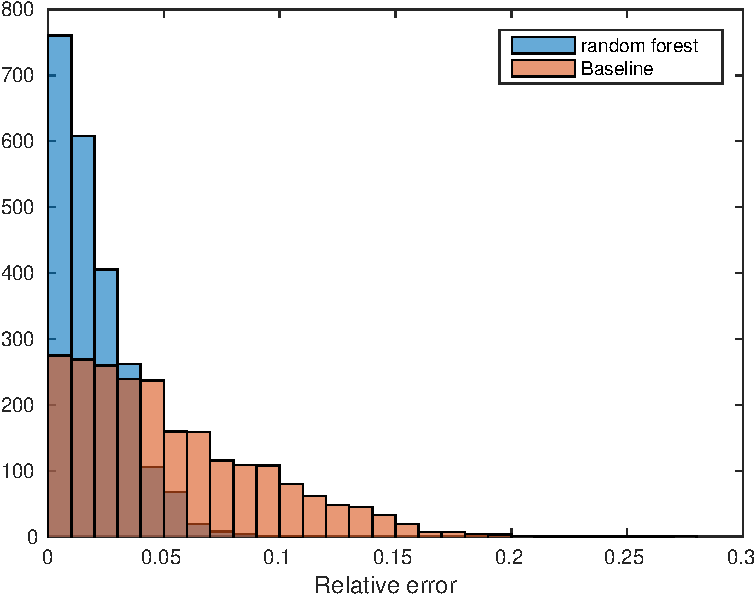
\includegraphics[width=0.3\linewidth]{figures/histogram_random_forest.pdf}
   }
   \caption{Relative error histograms of different estimators.}
   \label{fig:hist}
\end{figure}
